\documentclass{article}
\usepackage{listings}
\usepackage{mathrsfs}
\usepackage[utf8]{inputenc}
\usepackage{amssymb}
\usepackage{lipsum}
\usepackage{amsmath}
\usepackage{fancyhdr}
\usepackage{geometry}
\usepackage{scrextend}
\usepackage[english,german]{babel}
\usepackage{titling}
\setlength{\droptitle}{-3cm}
\usepackage{tikz}
\usepackage{algorithm,algpseudocode}
\usepackage[doublespacing]{setspace}
\usetikzlibrary{datavisualization}
\usetikzlibrary{datavisualization.formats.functions}
\usepackage{polynom}
\usepackage{amsmath}
\usepackage{gauss}
\usepackage{tkz-euclide}
\usetikzlibrary{datavisualization}
\usetikzlibrary{datavisualization.formats.functions}
\author{
Alexander Mattick Kennung: qi69dube\\
Kapitel 1
}
\usepackage{import}
\date{\today}
\geometry{a4paper, margin=2cm}
\usepackage{stackengine}
\parskip 1em
\newcommand\stackequal[2]{%
  \mathrel{\stackunder[2pt]{\stackon[4pt]{=}{$\scriptscriptstyle#1$}}{%
  $\scriptscriptstyle#2$}}
 }
\makeatletter
\renewcommand*\env@matrix[1][*\c@MaxMatrixCols c]{%
  \hskip -\arraycolsep
  \let\@ifnextchar\new@ifnextchar
  \array{#1}}
\makeatother
\lstset{
  language=haskell,
}
\lstnewenvironment{code}{\lstset{language=Haskell,basicstyle=\small}}{}
\usepackage{enumitem}
\setlist{nosep}
\usepackage{titlesec}
\usepackage{ stmaryrd }
\usepackage{verbatim}


\titlespacing*{\subsection}{0pt}{2pt}{3pt}
\titlespacing*{\section}{0pt}{0pt}{5pt}
\titlespacing*{\subsubsection}{0pt}{1pt}{2pt}
\title{Vorlesung 4}


\begin{document}
	\maketitle
	a)\\
	\[f_X(\alpha) = C\cdot 1_{(\frac{\pi}{9},\frac{5\pi}{18})}(\alpha)\]
	für eine Wahrscheinlichkeitsdichtefunktion muss $F(x)|_{-\infty}^{\infty}=1$ sein.\\
	\[\int^\infty_{-\infty}f_X(\alpha)d\alpha= 1\]
	\[\int^\infty_{-\infty}C\cdot 1_{(\frac{\pi}{9},\frac{5\pi}{18})}(\alpha)d\alpha=1\]
	\[\int^{\frac{5\pi}{18}}_{\frac{\pi}{9}}Cd\alpha=1\]
	\[C\cdot \frac{5\pi}{18}-C\cdot\frac{\pi}{9}=1\]
	\[C=\frac{6}{\pi}\]
	b)\\
	zuerst müssen die dazugehörigen $\alpha$ Werte bestimmt werden:\\
	\[35m = \frac{(20\frac{m}{s})^2}{10\frac{m}{s^2}}\sin(2\alpha)\]
	\[35m = \frac{(20\frac{m}{s})^2}{10\frac{m}{s^2}}\sin(2\alpha)\]
	\[35m\frac{10\frac{m}{s^2}}{(20\frac{m}{s})^2} = \sin(2\alpha)\]
	\[\frac{7}{8} = \sin(2\alpha)\]
	Dazu $\sin^{-1}(\frac{7}{8})/2=\alpha\implies \alpha\approx 0.5327$\\
	Wir betrachten hier nur Lösungen im bereich $\Omega = [0,\frac{\pi}{2}]$\\
	also
	\[\alpha_1 = \sin^{-1}(\frac{7}{8})/2\approx 0.5327\]
	\[\alpha_1 = \frac{\pi}{2}-\frac{\sin^{-1}(\frac{7}{8})}{2}\approx 1.0380\]
	in diesem intervall ist nun $W(\alpha)\geq 35[m]$.\\
	Dies jetzt in die Wahrscheinlichkeitsdichtefunktion eingesetzt:
	\[P(\sin^{-1}(\frac{7}{8})/2\leq \alpha\leq\frac{\pi}{2}-\frac{\sin^{-1}(\frac{7}{8})}{2})=\]
	\[\int^{\frac{\pi}{2}-\frac{\sin^{-1}(\frac{7}{8})}{2}}_{\sin^{-1}(\frac{7}{8})/2}f_X(\alpha)\]
	\[\int^{\frac{\pi}{2}-\frac{\sin^{-1}(\frac{7}{8})}{2}}_{\sin^{-1}(\frac{7}{8})/2}\frac{6}{\pi}1_{(\frac{\pi}{9},\frac{5\pi}{18})}(\alpha)d\alpha\]
	\[\int^{\frac{5\pi}{18}}_{\sin^{-1}(\frac{7}{8})/2}\frac{6}{\pi}d\alpha\]
	\[(\frac{5\pi}{18})*\frac{6}{\pi}-\sin^{-1}(\frac{7}{8})/2*\frac{6}{\pi}\]
	\[(\frac{5*6}{18})-\sin^{-1}(\frac{7}{8})/2*\frac{6}{\pi}\]
	mit exakten werten erhält man $\approx 0.6492504$\\
	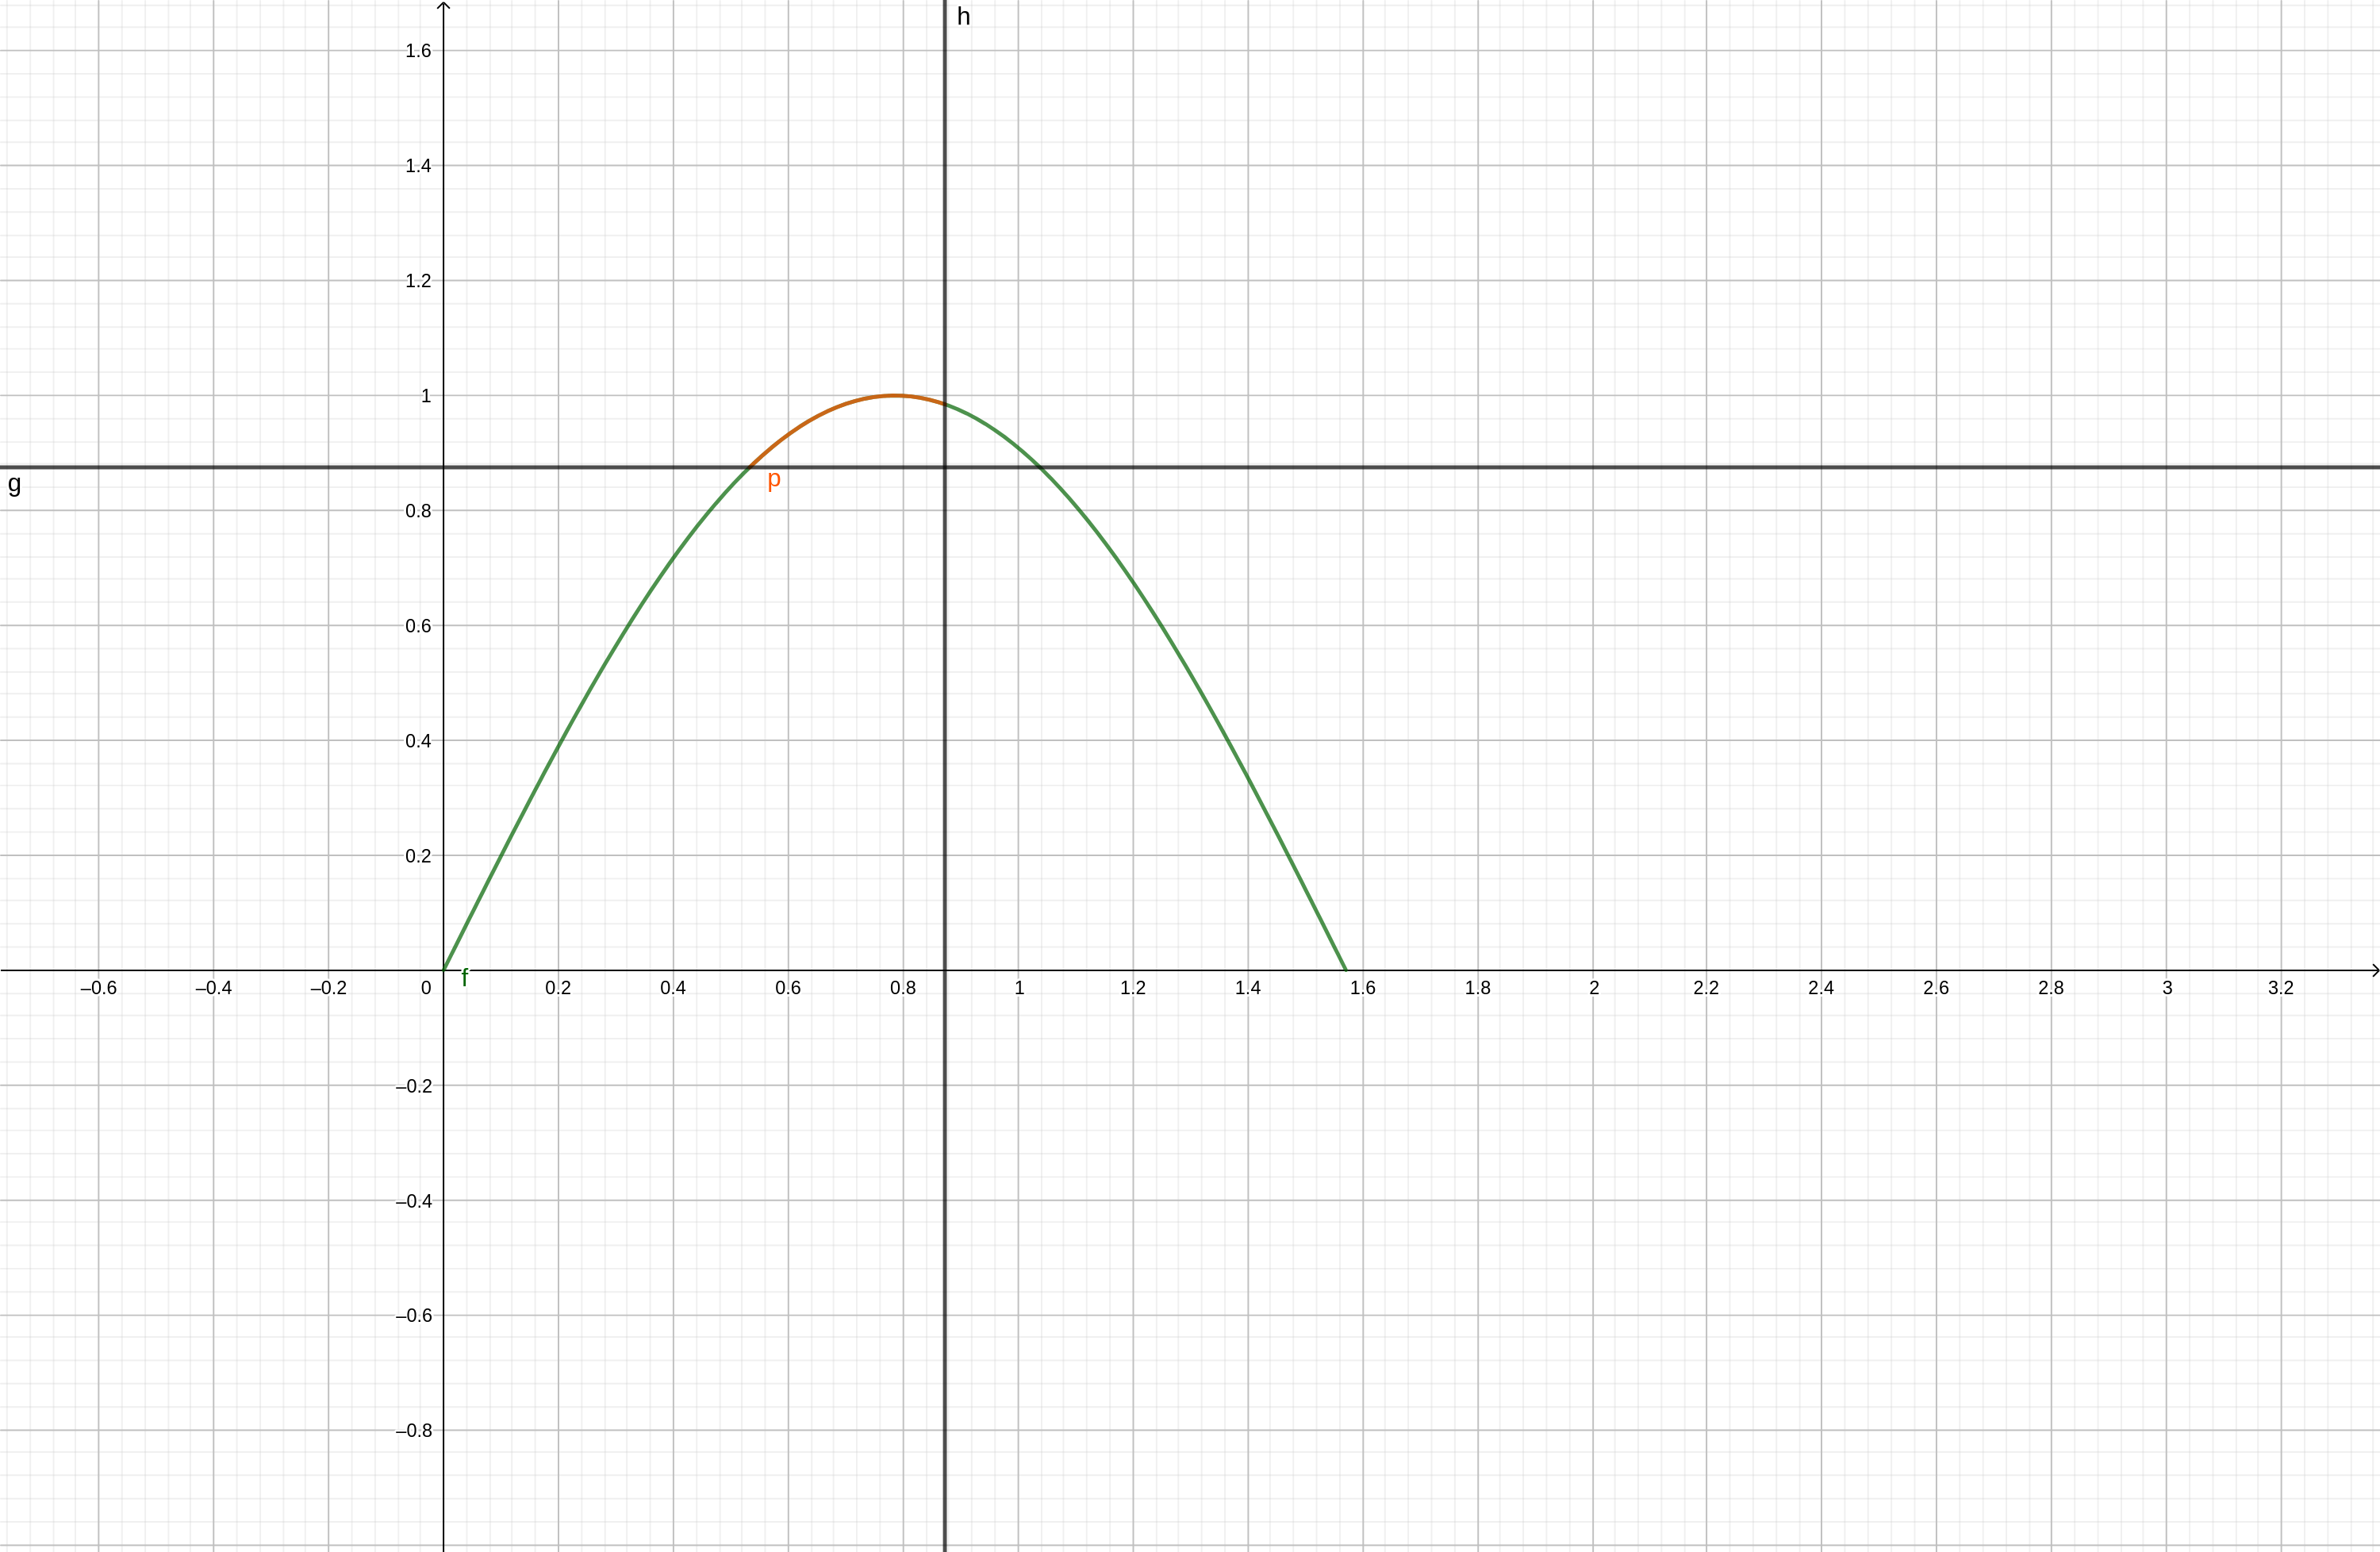
\includegraphics[width=256px]{SPs.png}\\
	c)\\
	Wie in der Zeichnung zu b) gesehen, gibt es eine Maximalstelle, nach der es wieder nach unten geht (also bereits erzielte Wurfweiten erneut erzielt werden).\\
	Dieser Punkt ist bei:\\
	\[\frac{v_0^2}{g}\sin(2\alpha)d/d\alpha\stackrel{!}{=} 0\]
	\[2\frac{v_0^2}{g}\cos(2\alpha)\stackrel{!}{=} 0\]
	\[\cos(2\alpha)\stackrel{!}{=} 0\]
	\[\alpha = \frac{n\pi}{2}-\frac{\pi}{4}, n\in\mathbb{Z}\]
	Der einzige Hochpunkt mit $\alpha\in[0,\frac{\pi}{2}]$ ist $n=1\implies \frac{\pi}{4}$\\
	Ab diese haben wir die doppelte wahrscheinlichkeit im Interval $(\frac{\pi}{9},\frac{5\pi}{18})$\\
	\[f^W(w)=\begin{cases}
	\frac{6}{\pi}&W(\frac{\pi}{9})<w<W(\frac{5\pi}{18})\\
	\frac{2*6}{\pi}&W(\frac{\pi}{4})\geq w\geq W(\frac{5\pi}{18}) \\
	0&sonst
	\end{cases}\]
	mit $W(\alpha)=\frac{15^2}{10}\sin(2\alpha)$
	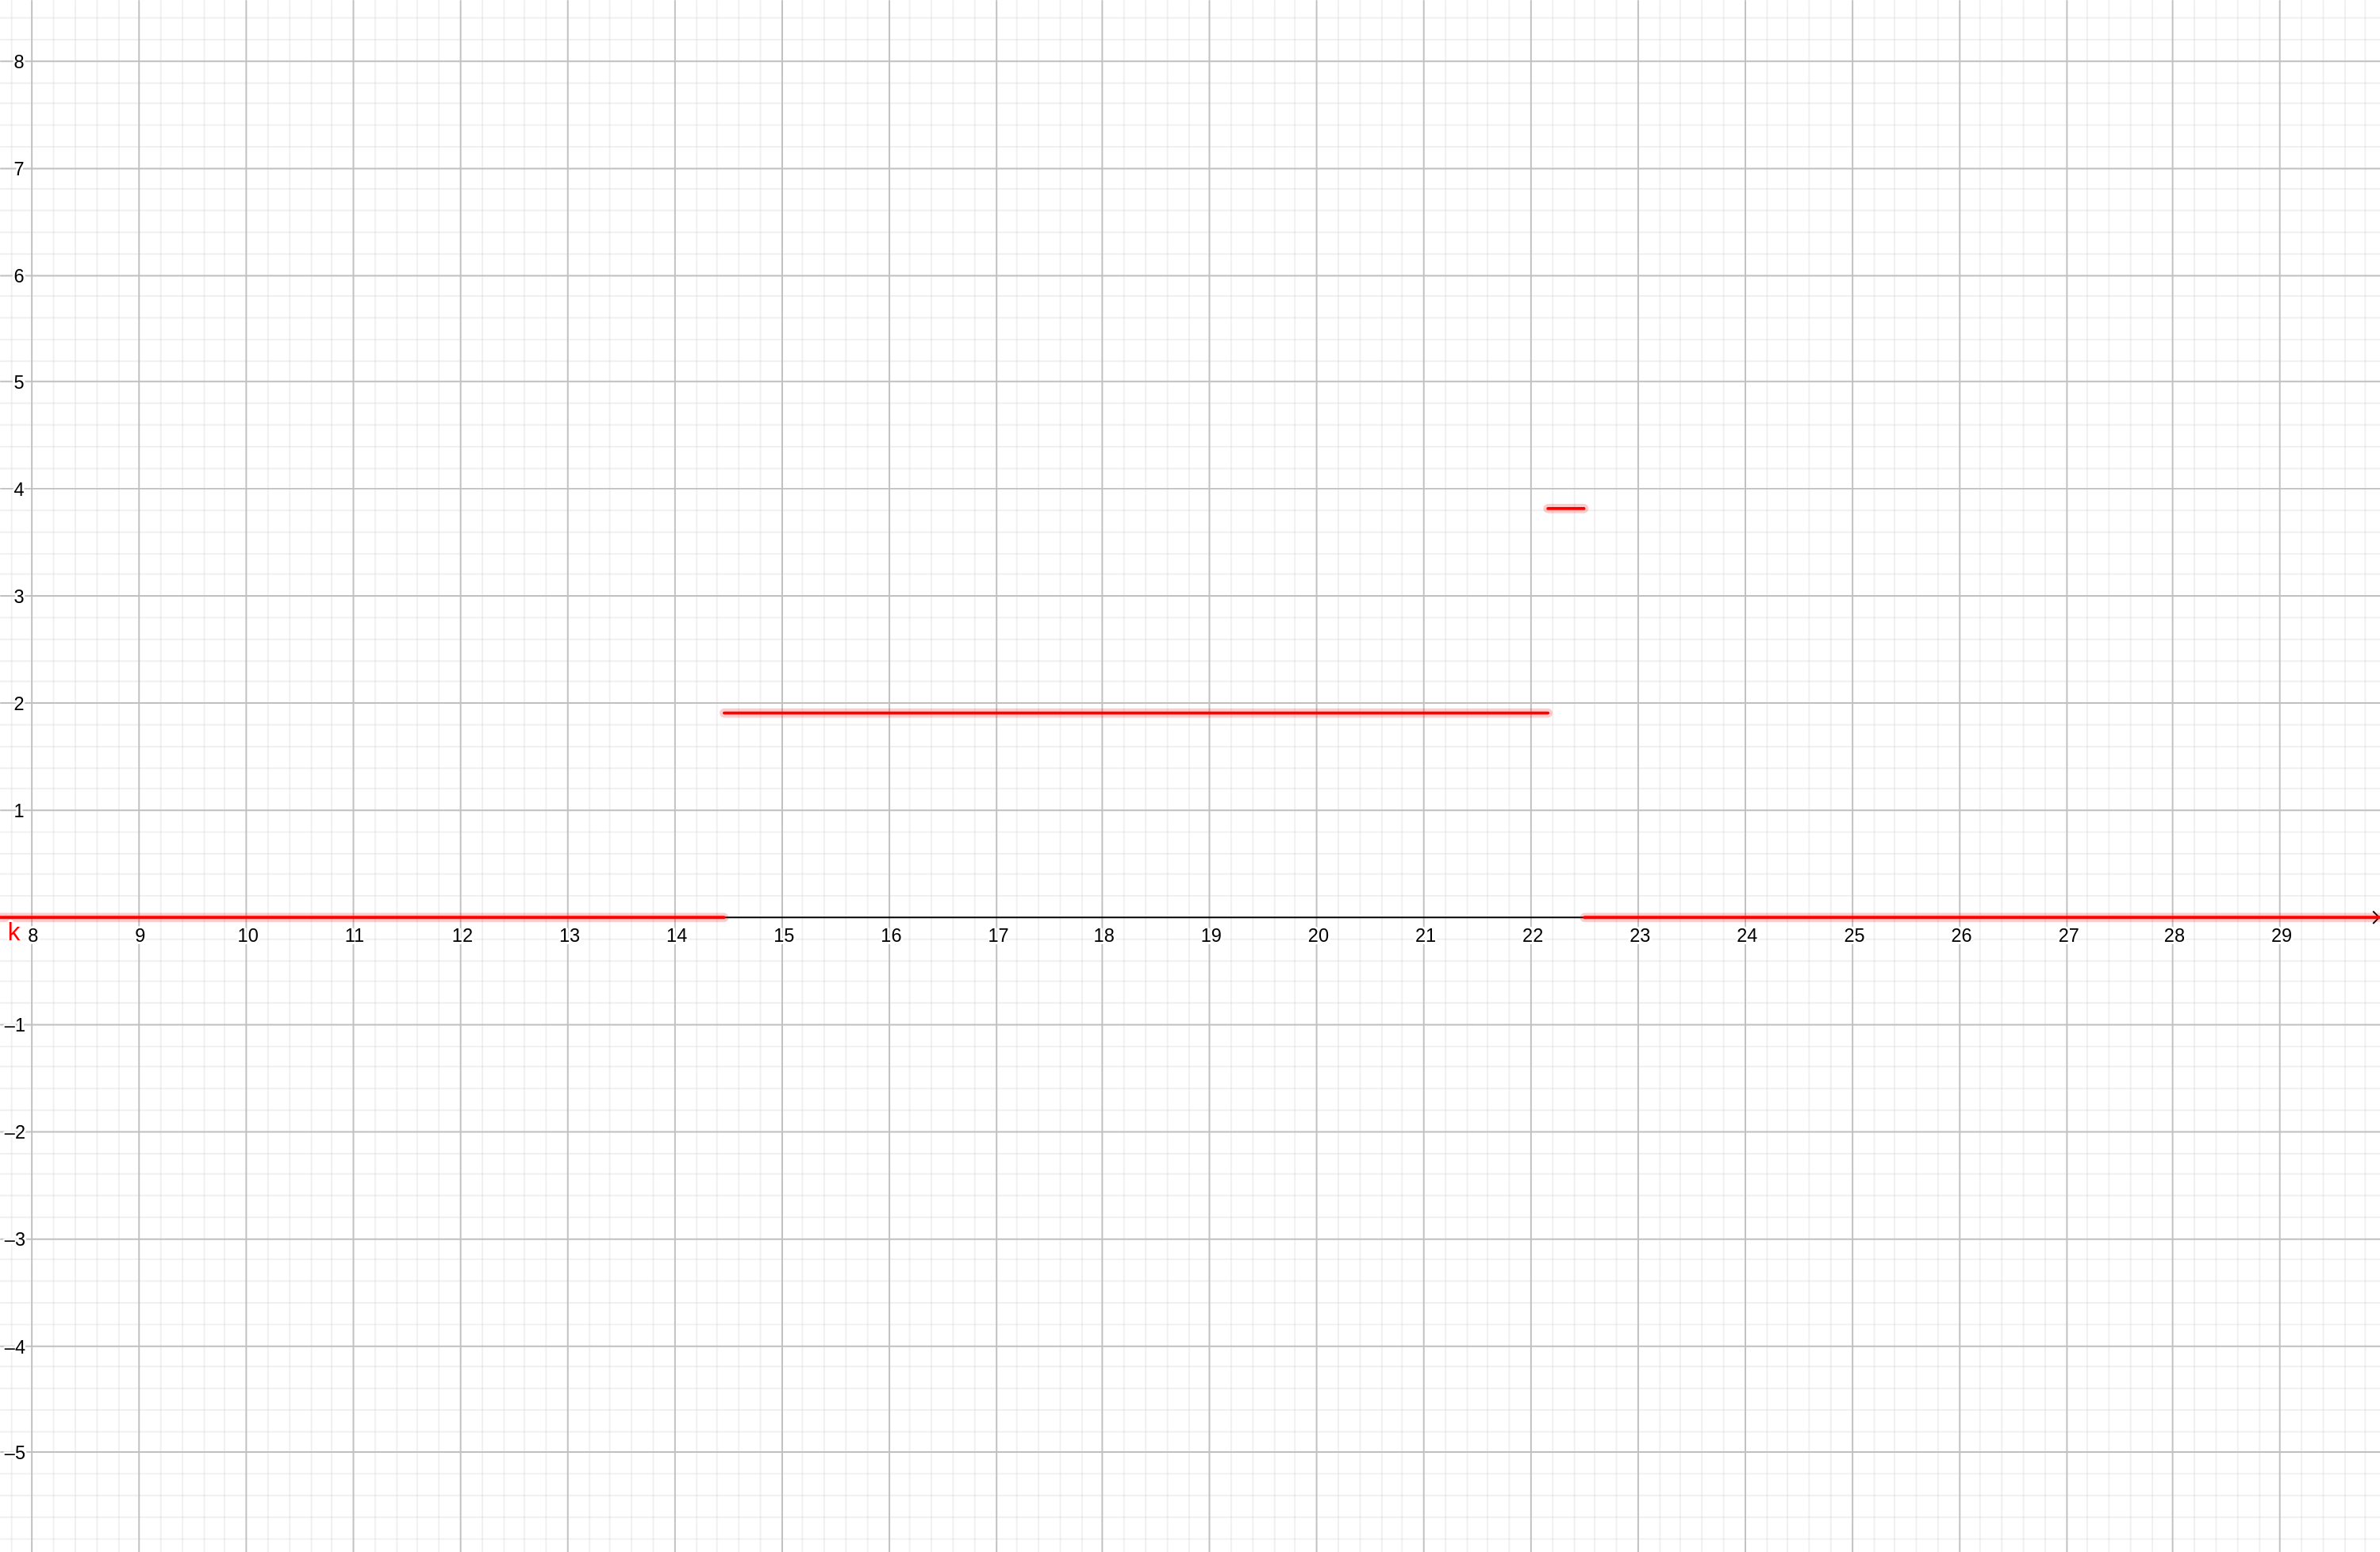
\includegraphics[height=256px]{intervalle.png}
	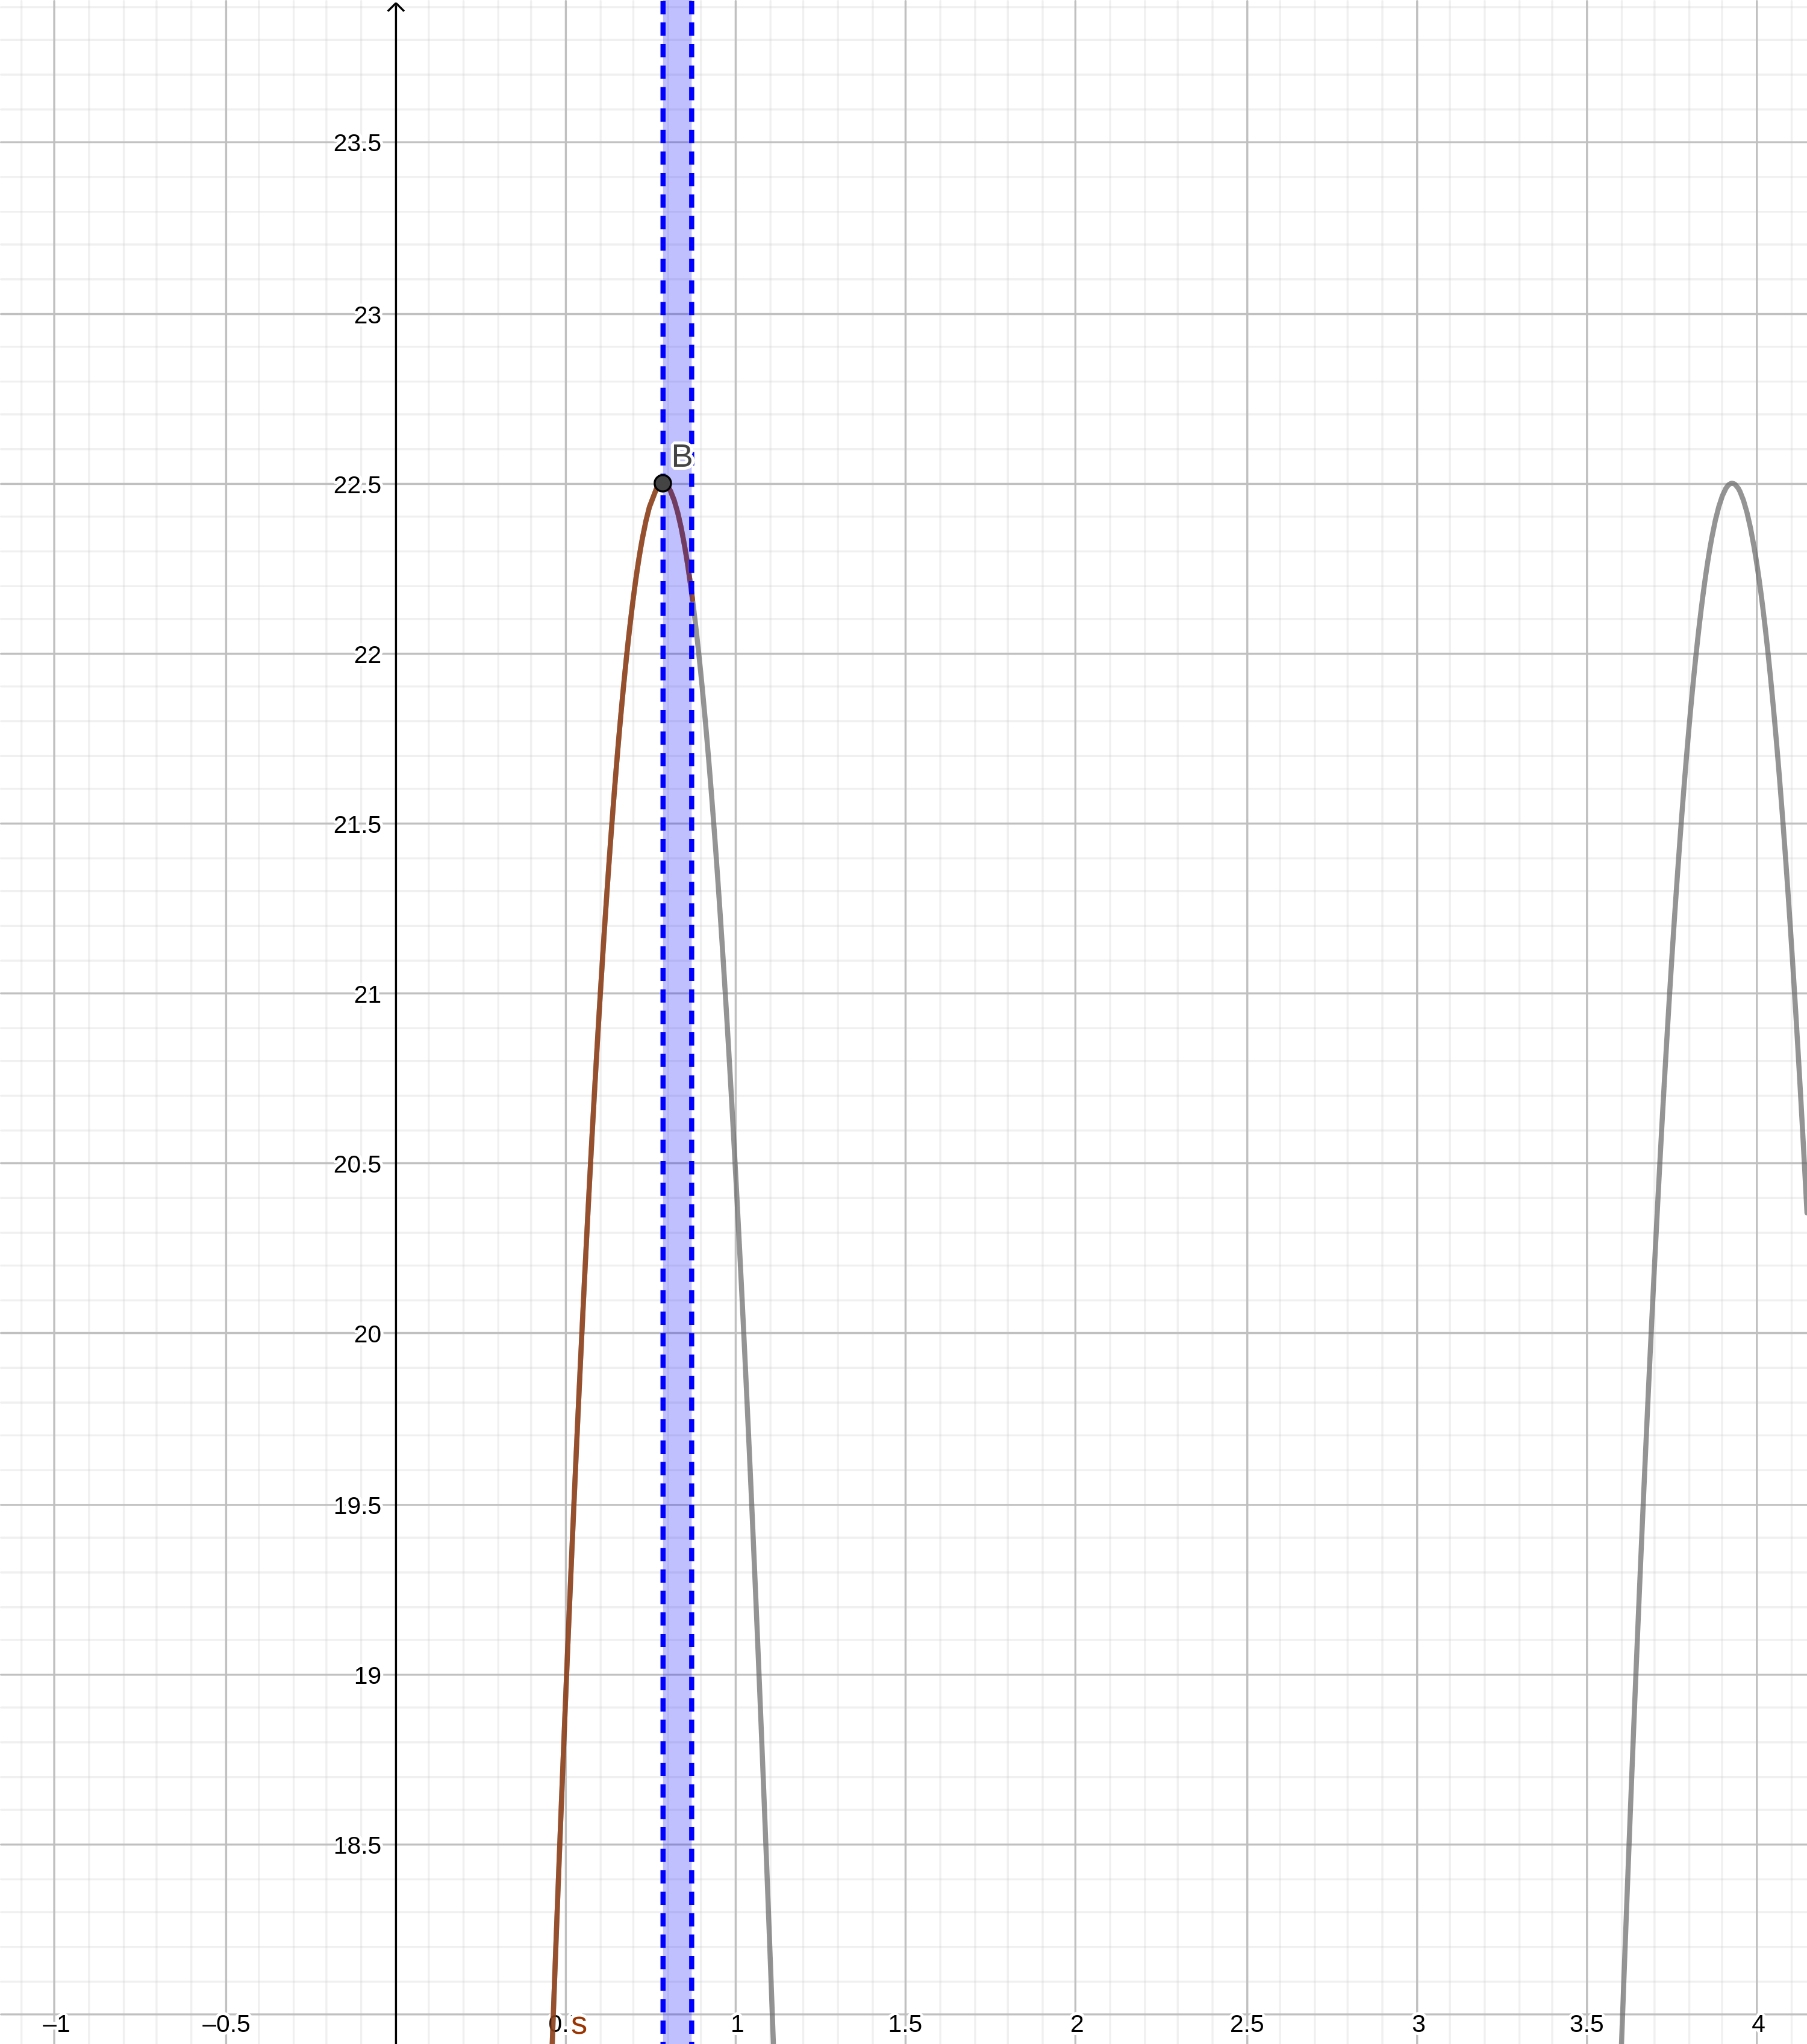
\includegraphics[height=256px]{gezeigtNichtNullIntervall.png}

\end{document}